\chapter{Introducción}

\section{Programa FORTE}

\drop{E}{ste} \acf{TFG} se ha desarrollado enmarcado en un convenio \acf{FORTE} con la empresa Intelygenz, el cuál forma parte del programa prefESIonalizate de la \acf{ESI} de Ciudad Real. Este
convenio permite la realización del TFG mientras se realizan prácticas en empresas.

\section{Inteligenz}

En Intelygenz~\ref{fig:intelygenz} es una empresa con sedes en San Francisco y Madrid, que se dedica al desarrollo de software a medida.  También 
desarrolla productos propios como Terminus7, Nextinit o HonestCode. Y trabajan con empresas como BBVA, Vodafone, BMW o Dolby. 

\begin{figure}[!h]
	\begin{center}
		
\includegraphics[width=0.4\textwidth]{./img/introduccion/intelygenz.jpg}
		\caption{Logo de Intelygenz}
		\label{fig:intelygenz}
	\end{center}
\end{figure}

\section{Sistema de Administración de Ideas}
En  la actualidad, cada vez es más frecuente escuchar hablar del talento humano de las empresas. Éste es el mejor recurso de estas,
 los empleados son los que mejor conocen su trabajo y pueden tener ideas de como mejorar diversos aspectos de la empresa. 
 
 Los clásicos buzones de sugerencias pueden servir a las empresas para conocer las mayores molestias de
  algunos de sus empleados. Estos rápidamente pueden convertirse en buzones de quejas, o los empleados pueden
   sentir que no se toman en cuenta sus opiniones si estas  sugerencias o quejas no obtienen una respuesta.
 
 Un \acf{SMI} puede ayudar a las empresas a fomentar la innovación desde cualquiera de los miembros de 
 estas. Además, «contar con información sobre la opinión de los empleados permite evitar errores en la toma
  de decisiones, y ayuda a dirigir los esfuerzos de mejora allí donde la organización detecta problemas»
   \cite{talento}. Los principales beneficios de estos sistemas son:
 
 \begin{itemize}
 	\item Aumento del compromiso de los empleados. 
 	\item Promueve la transparencia dentro de la empresa. Cada una de los miembros de la organización
 	puede aportar sus ideas sin necesidad de pasar por 	su «jefe». Todos los usuarios tienen la misma
 	 importancia y visibilidad.
 	\item Permite a los empleados dar su opinión. Todos los empleados en la compañía pueden proponer sus  ̈cambios y mejoras en Nextinit.
 	\item Detecta el talento. La organización detecta cuáles de sus miembros tienen
 	mayor talento para llevar a cabo esas iniciativa de mejora planteadas en la herramienta.
 	\item Retiene el talento. Nextinit ayuda a retener el talento, pues los miembros de la organización
 	 ven como sus propuestas son tomadas en consideración y como aquellas que han conseguido el apoyo de
 	  sus compañeros se implantan.
 	\item Mejora el clima laboral. Nextinit hace que los miembros de la organización colaboren entre sí 
 	para sacar adelante las ideas, por tanto mejora el clima laboral.
 	\item Alinea todos los empleados con los objetivos estratégicos de la compañía. La empresa puede definir cuales son sus prioridades estratégicas en Nextinit, de tal manera que cada una de las ideas 
 	cumplirá un porcentaje de cada una de las prioridades estratégicas establecidas (ver Figura~\ref{fig:prioridades}).
 	\item Genera ideas apoyadas por los empleados para mejorar la empresa en ámbitos muy diversos.
 \end{itemize}

\begin{figure}[!h]
	\begin{center}
		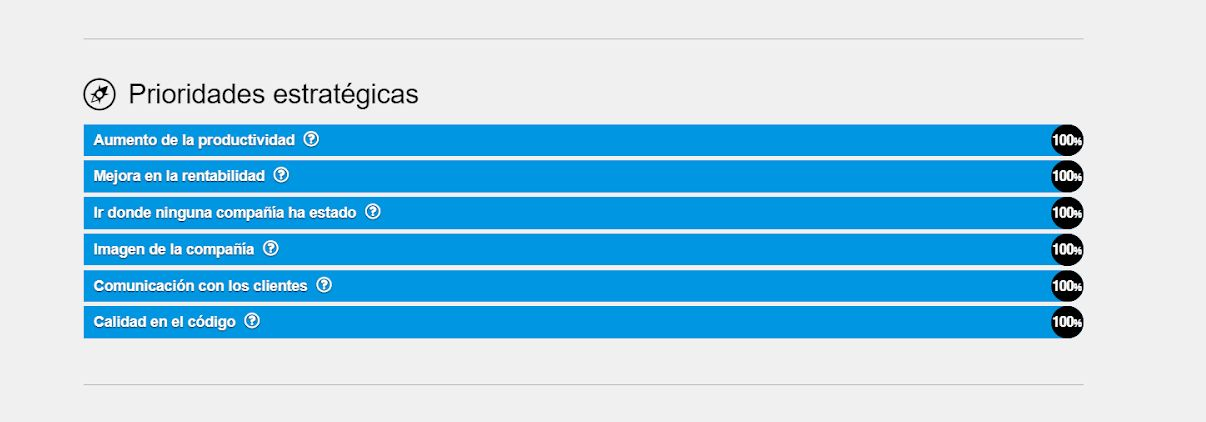
\includegraphics[width=0.8\textwidth]{./img/introduccion/prioridades.png}
		\caption{Ejemplo de prioridades estratégicas en Nextinit}
		\label{fig:prioridades}
	\end{center}
\end{figure}
  
 
\section{Estructura del documento}

El presente documento se compone con la siguiente estructura:

\begin{definitionlist}
\item[Capítulo \ref{chap:objetivos}: \nameref{chap:objetivos}] Se expone el objetivo principal y sus subjetivos.
 \item[Capítulo \ref{chap:antecedentes}: \nameref{chap:antecedentes}] Se describen los sistemas tomados como referencia utilizados para 
 el desarrollo de este \acs{TFG}.
  \item [Capítulo \ref{chap:metodo}: \nameref{chap:metodo}] Se describe y justifica la metodología utilizada para el desarrollo de este \acs{TFG}.
  \item[Capítulo \ref{chap:resultados}: \nameref{chap:resultados}] Se muestran los resultado obtenidos al aplicar la metodología elegida.
  \item[Capítulo \ref{chap:conclusiones}: \nameref{chap:conclusiones}] Se exponen las conclusiones llegadas al finalizar el desarrollo.
\end{definitionlist}

% Local Variables:
%  coding: utf-8
%  mode: latex
%  mode: flyspell
%  ispell-local-dictionary: "castellano8"
% End